\documentclass[12pt,english,spanish,noprefix,refpage]{book}
\usepackage{lmodern}
\renewcommand{\sfdefault}{lmss}
\renewcommand{\ttdefault}{lmtt}
\renewcommand{\familydefault}{\sfdefault}
\usepackage[T1]{fontenc}
\usepackage[latin9]{inputenc}
\usepackage{geometry}
\geometry{verbose,tmargin=2cm,bmargin=2cm,lmargin=2.5cm,rmargin=2cm}
\setcounter{secnumdepth}{3}
\setcounter{tocdepth}{3}
\usepackage{calc}
\usepackage{textcomp}
\usepackage{csquotes}
\usepackage{booktabs}
\usepackage{pgfgantt}
\usepackage{array}
\usepackage{wrapfig}
\usepackage{tabularx}
\usepackage{graphicx}
\usepackage{setspace}
\usepackage[authoryear]{natbib}
\usepackage{nomencl}
% the following is useful when we have the old nomencl.sty package
\providecommand{\printnomenclature}{\printglossary}
\providecommand{\makenomenclature}{\makeglossary}
\makenomenclature
\onehalfspacing
\definecolor{barblue}{RGB}{153,204,254}
\definecolor{groupblue}{RGB}{51,102,254}
\definecolor{linkred}{RGB}{165,0,33}
\makeatletter
\raggedbottom

%%%%%%%%%%%%%%%%%%%%%%%%%%%%%% LyX specific LaTeX commands.
%% Because html converters don't know tabularnewline
\providecommand{\tabularnewline}{\\}

%%%%%%%%%%%%%%%%%%%%%%%%%%%%%% User specified LaTeX commands.
\usepackage{algorithmic}
\usepackage{algorithm}
\floatname{algorithm}{Algoritmo}
\usepackage{layout}
\floatname{table}{Tabla}
\usepackage{url}
\usepackage{hyperref}
\usepackage{fancyhdr}
\fancyhf{}
\setlength{\headheight}{15.2pt}
\pagestyle{fancy}
\renewcommand{\chaptermark}[1]{\markboth{#1}{}}
\renewcommand{\sectionmark}[1]{\markright{#1}{}}
\makeatletter
\let\sv@endpart\@endpart
\def\@endpart{\thispagestyle{empty}\sv@endpart}
\makeatother

\makeatother

\usepackage{babel}
\addto\shorthandsspanish{\spanishdeactivate{~<>}}

\usepackage{listings}
\addto\captionsenglish{\renewcommand{\lstlistingname}{Listing}}
\addto\captionsspanish{\renewcommand{\lstlistingname}{Listado de c�digo}}
\renewcommand{\lstlistingname}{Listado de c�digo}

\begin{document}
\begin{titlepage}\thispagestyle{empty}%
\fbox{\begin{minipage}[c][0.99\textheight][t]{0.95\columnwidth}%
\vspace{1cm}
\begin{center}

\includegraphics[width=2cm]{figs/escudo_uned}
\par\end{center}
\bigskip{}
\begin{singlespace}
\begin{center}
{\large{}UNIVERSIDAD NACIONAL DE EDUCACI�N A DISTANCIA}\vspace{0.7cm}
\par\end{center}
\begin{center}
{\large{}ESCUELA T�CNICA SUPERIOR DE INGENIER�A INFORM�TICA}\vspace{0.5cm}
\par\end{center}
\begin{center}
Proyecto de Fin de Grado en Ingenier�a en Tecnolog�as de la Informaci�n {\Large{}\vspace{0.8cm}
}
\par\end{center}{\Large \par}
\end{singlespace}
\begin{center}
\textbf{\Large{}RDFplay: UN PLAYGROUND }\\
\textbf{\Large{}PARA FORMACI�N EN TECNOLOG�AS}\\
\textbf{\Large{}DE LA WEB SEM�NTICA}
\par\end{center}{\Large \par}
\vfill{}
\begin{flushleft}
\qquad{}MIGUEL EXP�SITO MART�N\bigskip{}
\par\end{flushleft}
\begin{flushleft}
\qquad{}Dirigido por: JOS� LUIS FERN�NDEZ VINDEL
\par\end{flushleft}
\begin{flushleft}
\qquad{}Co-dirigido por: RAFAEL MART�NEZ TOM�S
\par\end{flushleft}
\begin{flushleft}
\vspace{1.5cm}
\par\end{flushleft}
\begin{flushleft}
\qquad{}Curso: 2017-2018: 2� Convocatoria
\par\end{flushleft}
\bigskip{}
%
\end{minipage}}

\end{titlepage}
\thispagestyle{empty}

\cleardoublepage{}

\thispagestyle{empty}%
\fbox{\begin{minipage}[c][0.99\textheight][t]{0.95\columnwidth}%
\begin{center}
\vspace{1cm}
\par\end{center}
\begin{center}

\includegraphics[width=2cm]{figs/escudo_uned}
\par\end{center}
%\bigskip{}
\begin{singlespace}
\begin{center}
\textbf{\Large{}DESARROLLO DE UN PLAYGROUND }\\
\textbf{\Large{}PARA FORMACI�N EN TECNOLOG�AS}\\
\textbf{\Large{}DE LA WEB SEM�NTICA}
\par\end{center}{\large \par}
\end{singlespace}
\begin{center}
Proyecto de Fin de Grado de modalidad oferta espec�fica
\par\end{center}
\begin{flushleft}
\vspace{0.3cm}
\par\end{flushleft}
\begin{flushleft}
\enskip{}Realizado por:{\large{}\hspace{0.5em}}Miguel Exp�sito Mart�n{\large{}}
\vspace{0.3cm}
\par\end{flushleft}
\begin{flushleft}
\enskip{}Dirigido por:{\large{}\hspace{0.5em}}Jos� Luis Fern�ndez Vindel
\par\end{flushleft}
\begin{flushleft}
\enskip{}Co-dirigido por:{\large{}\hspace{0.5em}}Rafael Mart�nez Tom�s
\par\end{flushleft}
\begin{flushleft}
{\large{}}\vspace{0.6cm}
\par\end{flushleft}
\begin{flushleft}
\enskip{}Tribunal calificador
\par\end{flushleft}
\begin{flushleft}
\enskip{}Presidente: D/D�. 
\par\end{flushleft}
\begin{flushleft}
\textbf{\medskip{}
}
\par\end{flushleft}
\noindent \begin{flushleft}
\enskip{}Secretario: D/D�. 
\par\end{flushleft}
\begin{flushleft}
\textbf{\medskip{}
}
\par\end{flushleft}
\noindent \begin{flushleft}
\enskip{}Vocal: D/D�. 
\par\end{flushleft}
\vfill{}
\begin{flushleft}
\enskip{}Fecha de lectura y defensa: 2/10/2018
\par\end{flushleft}
\begin{flushleft}
\enskip{}Calificaci�n: 
\par\end{flushleft}
\smallskip{}
%
\end{minipage}}
\thispagestyle{empty}


\chapter*{Agradecimientos}
\begin{center}
\thispagestyle{empty}
\par\end{center}

A mi familia, a mis amigos, a mi Director de proyecto y a los que, sin querer, me animaron a afrontar este reto.


\thispagestyle{empty}

\cleardoublepage{}

\pagenumbering{roman}\fancyhead[LE,RO]{\thepage}\fancyhead[LO]{\nouppercase{\leftmark}}\fancyhead[RE]{\nouppercase{\rightmark}}\noindent \begin{center}
\textbf{\Large{}Resumen}
\par\end{center}{\Large \par}
\setlength{\parskip}{\baselineskip}
\thispagestyle{empty}

El presente proyecto tiene como objeto el desarrollo de un sistema de \textit{playground} para SPARQL y RDF que habr� de servir como herramienta educativa de introducci�n a las tecnolog�as de la Web Sem�ntica. Su prop�sito es facilitar una interfaz de uso sencilla para que usuarios profanos puedan introducirse en este tipo de tecnolog�as a un nivel b�sico, permitiendo la realizaci�n de actividades acad�micas sobre manejo sencillo de grafos as� como sobre consultas SPARQL al conjunto de datos de trabajo o a \textit{endpoints} externos.

Si bien es cierto que la Web Sem�ntica alcanza hoy en d�a un estado de madurez razonablemente avanzado, el ritmo de cambio de las tecnolog�as de \textit{frontend} en \textit{Javascript} (en adelante, JS) es, cuanto menos, vertiginoso. Unido a ello, se tiene que la mayor parte de las implementaciones de componentes de la Web Sem�ntica han sido desarrolladas en tecnolog�as de \textit{backend} como \textit{Java} (\textit{Apache Jena}) o \textit{Python} (\textit{rdflib}), no existiendo a�n est�ndares o implementaciones maduras puramente en Javascript.

Se abordan, por tanto, tres retos: la necesidad de conseguir un producto sencillo y f�cilmente utilizable por usuarios no expertos, la dificultad para encontrar componentes maduros que a�nen Web Sem�ntica con \textit{frontend} y la conveniencia de apostar por un \textit{framework} de desarrollo en \textit{Javascript} estable y con una curva de aprendizaje suave.

Para dar soluci�n a estos problemas, se ha optado por desarrollar una  \textit{Single Page Application} (SPA) con Vue.js (un \textit{framework} JS que se jacta de aglutinar las mejores caracter�sticas de Angular y React, sus principales competidores en el mercado) e integrarlo con las implementaciones recomendadas por el grupo de trabajo de bibliotecas \textit{Javascript} \textit{rdfjs} y con una plataforma de consultas para la web flexible y modular. El sistema est� planteado para ejecutarse en un sencillo navegador contempor�neo, descarg�ndose a trav�s de un simple servidor web (siendo este la �nica infraestructura necesaria para su distribuci�n).

Dado el alto nivel de incertidumbre existente a la hora de implementar las necesidades del proyecto, se ha optado por utilizar un enfoque metodol�gico incremental e iterativo basado en \textit{Extreme Programming} y apoyado sobre tableros Kanban, lo que ha permitido una mejor organizaci�n y evoluci�n del proyecto.

El resultado final ofrece un producto b�sico de introducci�n a las tecnolog�as de la Web Sem�ntica y permite pensar en un desarrollo del mismo tan ambicioso como las propias necesidades de los equipos docentes, dado el estado de madurez actual del \textit{frontend} web.\thispagestyle{empty}

\selectlanguage{english}%
\noindent \begin{center}
\textbf{\Large{}Abstract}
\par\end{center}{\Large \par}

\noindent \thispagestyle{empty}

<This project ...>\selectlanguage{spanish}%

\thispagestyle{empty}

\cleardoublepage{}

\tableofcontents{}\cleardoublepage{}\markboth{\nomname}{\nomname}

\printnomenclature{}

\listoffigures

\renewcommand{\listtablename}{�ndice de tablas} 

\listoftables

\cleardoublepage{}\fancyhf{}\pagenumbering{arabic}\pagestyle{fancy}\fancyhead[LE,RO]{\thepage}\fancyhead[LO]{\chaptername {} \thechapter. \leftmark}\fancyhead[RE]{\thesection. \rightmark}

\chapter{Introducci�n}

No cabe duda que uno de los retos a los que se enfrenta la Sociedad de la Informaci�n y del Conocimiento es la educaci�n, una de las mejores inversiones en el futuro de Europa. Seg�n la �ltima Comunicaci�n de la Comisi�n al Parlamento, al Consejo, al Comit� Econ�mico y Social Europeo y al Comit� de las Regiones\cite{comission01},  el uso de las TIC para prop�sitos educativos se queda atr�s, tanto en adopci�n como en competencias del profesorado. La innovaci�n en sistemas educativos, entendida como la adopci�n de nuevos servicios y herramientas por parte de las organizaciones educativas, puede mejorar los resultados formativos y la eficiencia.

Siendo una de las prioridades del Plan de Acci�n propuesto por la Comisi�n hacer mejor uso de la tecnolog�a digital para el aprendizaje y la ense�anza, parece apropiado que instituciones como la Universidad Nacional de Educaci�n a Distancia (UNED) en Espa�a y sus departamentos, como el de Inteligencia Artificial, se propongan aplicar los �ltimos avances tecnol�gicos para mejorar la calidad del sistema educativo y facilitar a los alumnos la adquisici�n de nuevas competencias digitales complejas.

Dentro de estas competencias se pueden encuadrar t�rminos como Web de Datos, Web Sem�ntica o Datos Enlazados, todos definidos por el padre de la Web, Tim Berners-Lee\cite{bernerslee01, bernerslee02}. No son m�s que la evoluci�n l�gica de la Web a la que todos estamos acostumbrados, pero entendida en su crecimiento como una soluci�n a los problemas de la ingente cantidad de datos no estructurados o inconexos que se genera al d�a en 2018 (seg�n Domo\cite{domo01}, 2,5 quintillones de bytes).
 
En concreto, este trabajo pretende acercar las tecnolog�as de la Web Sem�ntica al alumnado siguiendo las recomendaciones del  W3C RDFJS Community Group\cite{rdfw3ccg} a trav�s de una sencilla aplicaci�n puramente desarrollada en Javascript y lista para usar, que permita la exploraci�n de facilidades de modelado y consulta sobre un conjunto de datos predefinido o aportado por el propio alumno as� como la carga y realizaci�n de actividades simples propuestas por el profesorado.


La memoria de este proyecto se estructura en los siguientes cap�tulos:

\begin{itemize}
	\item \textbf{Cap�tulo 1. Introducci�n.}  Esta introducci�n.
	\item \textbf{Cap�tulo 2. La Web Sem�ntica.} Una presentaci�n de las tecnolog�as que conforman la Web Sem�ntica: datos enlazados, RDF y SPARQL.
	\item \textbf{Cap�tulo 3. Motivaci�n y objetivos.} Se exponen las razones que llevaron a la elecci�n de este proyecto en concreto, as� como las metas que se esperaban alcanzar.
	\item \textbf{Cap�tulo 4. Trabajos previos, estado actual y recursos.} Un estudio sobre el estado actual de las tecnolog�as en cuesti�n y los recursos que se estiman necesarios para llevar a cabo con �xito el proyecto.
	\item \textbf{Cap�tulo 5. Metodolog�a y planificaci�n.} Descripci�n de la metodolog�a de desarrollo de software a utilizar y an�lisis de las planificaciones llevada a cabo (inicial y efectiva).
	\item \textbf{Cap�tulo 6. An�lisis.} Se presenta un estudio de necesidades para el sistema de informaci�n concretadas en casos de uso detallados.
	\item \textbf{Cap�tulo 7. Dise�o.} Descripci�n de las distintas arquitecturas del sistema, as� como su estructura basada en componentes.
	\item \textbf{Cap�tulo 8. Implementaci�n y pruebas.} Detalles de implementaci�n en Javascript y de las pruebas unitarias y extremo a extremo llevadas a cabo.
	\item \textbf{Cap�tulo 9. Resultados.}
	\item \textbf{Cap�tulo 10. Conclusiones y l�neas futuras de trabajo.}
\end{itemize}\cleardoublepage{}

\cleardoublepage{}

\chapter{Metodolog�a}

\section{Elecci�n de la metodolog�a}

Para acometer este proyecto, se han valorado dos familias de metodolog�as de desarrollo de \textit{software}:

\begin{enumerate}
	\item Metodolog�as en cascada (\textit{Waterfall})
	\item Metodolog�as �giles (incrementales e iterativas)
\end{enumerate} 

La metodolog�a de desarrollo en cascada surgi� como idea en un art�culo de Winston W. Royce en 1970{\cite{royce01}}. Hist�ricamente, este modelo se ha extendido tanto en �mbitos acad�micos como profesionales, siendo estas sus principales caracter�sticas:

\begin{itemize}
	\item Gesti�n predictiva de proyectos llevada al software.
	\item Toma como modelo la forma de proceder en el resto de ingenier�as.
	\item Intenta llenar el vac�o del \textit{code \& fix}.
	\item Cada fase se realiza, en principio, una �nica vez.
	\item Cada fase produce un entregable que ser� entrada de la siguiente.
	\item Los entregables no son, en principio, modificables.
\end{itemize}

Es decir, se basa en la separaci�n entre dise�o y construcci�n (o entre creatividad y repetici�n).

La propuesta de Royce,tal y como se desprende de la lectura del art�culo original, describ�a el modelo en cascada como la \blockquote[{\cite{royce01}}]{descripci�n m�s simple} que solo funcionar�a para los proyectos m�s sencillos. Ir�nicamente, este mensaje malentendido ha sido el origen de la popularidad de la metodolog�a en cascada, que hoy en d�a se sigue promoviendo en muchos casos por inercia, desconocimiento, comodidad o ilusi�n de control sobre el proyecto.
 
Lamentablemente, en la \textit{Ingenier�a de Software} los pesos de dise�o y construcci�n est�n invertidos con respecto a otras ingenier�as, siendo el \textit{software} un dominio de cambio y alta inestabilidad. El desarrollo de \textit{software} es, intr�nsecamente, una labor creativa; y la creatividad no es f�cilmente predecible. Esto ha dado lugar a que los desarrollos tradicionales adolezcan de ciertos problemas{\cite{larman01}}:

\begin{itemize}
	\item Existencia de muchos requisitos vagos o especulativos y dise�o detallado por adelantado.
	\item Est�n fuertemente asociados con las tasas de fallo m�s altas en proyectos.
	\item Se encuentran promovidos hist�ricamente por creencia m�s que por evidencia estad�stica significativa.
	\item Su rigidez incrementa el riesgo de fracaso, pospuesto hasta las fases finales del proyecto.
	\item Asume que las especificaciones son predecibles, estables y completas.
	\item Pospone integraci�n y pruebas hasta fases tard�as.
	\item Se basa en estimaciones y planificaci�n ``fiables''.
\end{itemize}

Entre los estudios que ratifican las afirmaciones anteriores, cabe citar los siguientes:

\begin{itemize}
	\item Informe Chaos 2015\cite{chaos15}.
	\item \textit{Dr. Dobb's Journal article The Non'Existent Software Crisis: Debunking the Chaos Report}\cite{ambler01}.
	\item Encuesta de Gartner\cite{mieritz01}.
    \item TODO
\end{itemize}

Por tanto, atendiendo a esta exposici�n y considerando que el proyecto en cuesti�n presentaba un alto nivel de incertidumbre debido a su alto componente en investigaci�n del estado tecnol�gico actual, se ha optado por utilizar un enfoque metodol�gico incremental e iterativo, puesto que:

\begin{itemize}
	\item Facilita llevar a cabo proyectos peque�os.
	\item Fomenta la interacci�n entre el desarrollador y el usuario.
	\item Fuerza a que los inevitables cambios en requisitos sucedan en fases tempranas del proyecto.
\end{itemize}

Entre sus caracter�sticas es posible citar:

\begin{itemize}
	\item Se trabaja sobre subconjuntos de funcionalidad (\textit{features}).
	\item Los incrementos permiten a�adir funcionalidad al producto (mejora del proceso).
	\item Las iteraciones permiten redise�ar, revisar y refactorizar el producto (mejora del producto).
	\item Se basa en entregas frecuentes y ciclos prueba/error.
	\item Ofrece flexibilidad a la hora de gestionar el cambio.
\end{itemize}

La referencia m�s clara en este �mbito es \textit{Extreme Programming}, de Kent Beck\cite{beck01}. \textit{Extreme Programming} es \blockquote[{\cite{royce01}}]{un estilo de desarrollo de software centrado en la aplicaci�n excelente de t�cnicas de programaci�n, comunicaci�n clara y trabajo en equipo que permite conseguir objetivos antes impensables}. Se trata de una metodolog�a basada en valores como la comunicaci�n, realimentaci�n, simplicidad, valent�a y respeto, soportada sobre un cuerpo de pr�cticas �tiles y con un conjunto de principios complementarios, adem�s de contar con una comunidad de usuarios que comparte todo lo anterior.

Su aplicaci�n al desarrollo de este proyecto no ha sido estricta; por ejemplo, no se han definido ciclos estrictos por la propia naturaleza inestable de la dedicaci�n al desarrollo del mismo, pero s� que ha realizado un dise�o evolutivo soportado sobre un n�mero suficiente de pruebas unitarias as� como una planificaci�n incremental y adaptativa a las problem�ticas que iban surgiendo.

Prueba del acierto a la hora de elegir esta metodolog�a es el cambio de necesidades y requisitos funcionales que tuvo lugar en la reuni�n presencial mantenida con el tutor, donde \textbf{la metodolog�a aport� que no fuera necesario descartar ning�n desarrollo o trabajo realizado hasta la fecha}. Permiti� realizar una gesti�n del cambio efectiva, re-orientando el trabajo a tiempo sin impactar en el dise�o ni en la implementaci�n existente. Finalmente, tanto la organizaci�n como la planificaci�n de las tareas han sido lo suficientemente flexibles para conseguir un ritmo adecuado de desarrollo, reduciendo los puntos de bloqueo.
\cleardoublepage{}

\chapter{Planificaci�n}


\section{Planificaci�n global}

Para realizar la planificaci�n del proyecto, y dada la metodolog�a de desarrollo incremental e iterativa elegida, no se ha seguido un modelo t�pico en fases de \textit{An�lisis, Dise�o, Implementaci�n, etc.} sino que se ha optado por un enfoque orientado a tareas relacionadas con la funcionalidad del producto final esperado.

\begin{figure}[h]
\begin{ganttchart}[
	canvas/.append style={fill=none, draw=black!5, line width=.75pt},
	hgrid style/.style={draw=black!5, line width=.75pt},
	vgrid={*1{draw=black!5, line width=.75pt}},
	title/.style={draw=none, fill=none},
	title label font=\bfseries\footnotesize,
	title label node/.append style={below=4pt},
	include title in canvas=false,
	bar label font=\mdseries\small\color{black!70},
	bar label node/.append style={left=2cm},
	bar/.append style={draw=none, fill=black!63},
	bar incomplete/.append style={fill=barblue},
	bar progress label font=\mdseries\footnotesize\color{black!70},
	group/.append style={draw=none, fill=groupblue},
	group left shift=0,
	group right shift=0,
	group height=.5,
	group peaks tip position=0,
	group label node/.append style={left=.6cm},
	group progress label font=\bfseries\small,
	link/.style={-latex, line width=1.5pt, linkred},
	link label font=\scriptsize\bfseries,
	link label node/.append style={below left=-2pt and 0pt}
	]{1}{20}
	\gantttitle{Planificaci�n inicial}{20} \\
	\gantttitle{Febrero}{4}
	\gantttitle{Marzo}{4}
	\gantttitle{Abril}{4}
	\gantttitle{Mayo}{4}
	\gantttitle{Junio}{4}\\
	\gantttitle[
	title label node/.append style={below left=4pt and -3pt}
	]{Semana:\quad1}{1}
	\gantttitlelist{2,...,20}{1} \\
	\ganttgroup[]{Documentaci�n y arranque}{1}{4} \\
	\ganttgroup[]{Prueba de concepto}{4}{8} \\
	\ganttgroup[]{Desarrollo del proyecto}{8}{14} \\
	\ganttgroup[]{Resultados y memoria}{14}{20} \\
\end{ganttchart}
\caption{Planificaci�n inicial}\label{fig:gantt01}
\end{figure}

\pagebreak

La figura anterior (\ref{fig:gantt01}) muestra la planificaci�n propuesta para la elaboraci�n del anteproyecto.

En esta propuesta era clave la revisi�n de la prueba de concepto con el tutor para comprobar que efectivamente se hab�an comprendido las necesidades desprendidas del an�lisis y para poder continuar con la especificaci�n funcional de forma m�s refinada y precisa.

En la pr�ctica, la evoluci�n del proyecto ha sido bien distinta. En la figura \ref{fig:gantt02} se puede comprobar cu�l ha sido la planificaci�n efectiva, producto esta de cambios sobre la inicial para resolver los distintos imprevistos que han ido surgiendo durante la ejecuci�n del mismo.

\begin{figure}
	\begin{changemargin}{-1cm}{-1cm}
		\begin{tikzpicture}[y=0.50cm] 
		\begin{ganttchart}[
		y unit chart=0.8cm,
		canvas/.append style={fill=none, draw=black!5, line width=.75pt},
		hgrid style/.style={draw=black!5, line width=.75pt},
		vgrid={*1{draw=black!5, line width=.75pt}},
		title/.style={draw=none, fill=none},
		title label font=\bfseries\footnotesize,
		title label node/.append style={below=4pt},
		include title in canvas=false,
		bar label font=\mdseries\tiny\color{black!70},
		bar label node/.append style={left=0.5cm},
		bar/.append style={draw=none, fill=barblue!63},
		bar incomplete/.append style={fill=barblue},
		bar progress label font=\mdseries\footnotesize\color{black!70},
		group incomplete/.append style={fill=groupblue},
		group/.append style={draw=none, fill=groupblue},
		group left shift=0,
		group right shift=0,
		group height=.5,
		group peaks tip position=0,
		group label node/.append style={left=.6cm},
		group label font=\bfseries\tiny,
		milestone label font=\bfseries\tiny,
		link/.style={-latex, line width=1.5pt, linkred},
		link label font=\scriptsize\bfseries,
		link label node/.append style={below left=-2pt and -5pt}
		]{1}{28}
		\gantttitle{Planificaci�n efectiva}{28} \\
		\gantttitle{Febrero}{2}
		\gantttitle{Marzo}{4}
		\gantttitle{Abril}{4}
		\gantttitle{Mayo}{4}
		\gantttitle{Junio}{4}
		\gantttitle{Julio}{4}
		\gantttitle{Agosto}{4}
		\gantttitle{Septiembre}{2}\\
		\gantttitle[
		title label node/.append style={below left=4pt and -6pt}
		]{Semana:\quad1}{1}
		\gantttitlelist{2,...,28}{1} \\
		\ganttgroup[]{Formaci�n y arranque (FA)}{1}{6} \\
		\ganttbar[
		name=FA11
		]{\textbf{FA 1.1} RDF y OWL}{1}{2} \\
		\ganttbar[
		name=FA12
		]{\textbf{FA 1.2} JS ES6+, Vue}{3}{6} \\
		\ganttbar[
		name=FA13
		]{\textbf{FA 1.3} POC edici�n tripleta}{1}{6} \\
		\ganttmilestone{Prueba de concepto inicial}{6}{6} \\
		\ganttbar[
		name=FA14
		]{\textbf{FA 1.4} An�lisis de necesidades}{1}{6} \\
		\ganttgroup[]{Desarrollo de m�dulo de edici�n (ME)}{7}{20} \\
		\ganttbar[]{\textbf{ME 2.1} Plantilla Vue + testing}{7}{8} \\
		\ganttbar[]{\textbf{ME 2.2} Dise�o de componentes}{8}{9} \\
		\ganttbar[]{\textbf{ME 2.3} Implementaci�n CRUD clases}{9}{13} \\
		\ganttbar[]{\textbf{ME 2.4} Implementaci�n export/import}{12}{14} \\
		\ganttbar[]{\textbf{ME 2.5} Mejoras en visualizaci�n y uso }{14}{16} \\
		\ganttbar[]{\textbf{ME 2.6} Refactorizaci�n y generalizaci�n }{16}{20} \\
		\ganttbar[]{\textbf{ME 2.7} Pruebas}{7}{20} \\
		\ganttmilestone{Reuni�n presencial}{20}{20} \\
		\ganttgroup[]{Desarrollo de m�dulos playground}{20}{25} \\
		\ganttbar[]{\textbf{ME 3.1} M�dulo de consulta SPARQL}{20}{23} \\
		\ganttbar[]{\textbf{ME 3.2} M�dulo de carga de actividades}{23}{24} \\
		\ganttbar[]{\textbf{ME 3.3} M�dulo de carga de vocabularios}{23}{24} \\
		\ganttbar[]{\textbf{ME 3.4} Mejoras en la importaci�n}{23}{24} \\
		\ganttbar[]{\textbf{ME 3.5} Revisi�n, refactoring, cleaning}{24}{25} \\
		\ganttbar[]{\textbf{ME 3.6} Pruebas}{20}{25} \\
		\ganttgroup[]{Redacci�n de memoria y cierre}{24}{28} \\
		\ganttbar[]{\textbf{ME 4.1} Formaci�n latex}{24}{24} \\
		\ganttbar[]{\textbf{ME 4.2} Redacci�n memoria}{24}{28} \\
		
		\end{ganttchart}
		\end{tikzpicture}
	\end{changemargin}
	\caption{Planificaci�n efectiva}\label{fig:gantt02}
\end{figure}

Con respecto a la planificaci�n inicial, se tiene que:

\begin{itemize}
	\item El proyecto se ha retrasado un total de ocho semanas.
	\item El per�odo de formaci�n llev� al menos dos semanas m�s de lo esperado (en realidad, el aprendizaje del \textit{framework Vue} ha estado presente a lo largo de pr�cticamente todo el desarrollo del proyecto).
	\item El desarrollo del producto ha consumido seis semanas m�s de las previstas inicialmente.
	\item La memoria se ha redactado en dos semanas menos con respecto a la estimaci�n inicial.
\end{itemize} 

Las desviaciones surgidas con respecto a la planificaci�n inicial tienen su explicaci�n en los siguientes motivos:

\begin{itemize}
	\item El alto grado de incertidumbre a la hora de estimar la planificaci�n inicial, dado que se desconoc�a cu�l era la situaci�n actual del ecosistema tecnol�gico de \textit{front-end web} y su integraci�n con las tecnolog�as de la Web Sem�ntica.
	\item La curva de aprendizaje de \textit{Vue}, si bien es considerada m�s suave que la de sus competidores (\textit{React, Angular}) fue mayor de lo esperado. El bajo grado de familiarizaci�n del autor del proyecto con las tecnolog�as de \textit{front-end} y, especialmente, \textit{Javascript ES6+}, no facilit� el aprendizaje.
	\item El\textbf{ bajo nivel de madurez de las bibliotecas existentes} para la manipulaci�n de RDF en Javascript, as� como la heterogeneidad y poca estabilidad de estas implementaciones, ha suscitado muchas dudas sobre cu�les utilizar y c�mo enfocar su integraci�n con \textit{frameworks} m�s maduros como \textit{Vue}.
	\item La \textbf{pr�ctica ausencia de bibliotecas} o componentes de interacci�n con SPARQL \textbf{conformes a la especificaci�n est�ndar de la interfaz} \textit{rdf.js}{\cite{rdfjs01}} (que por otra parte, es un borrador de 2017) ha puesto en peligro la viabilidad del proyecto. La plataforma finalmente utilizada, \textit{Comunica}{\cite{comunica01}}, a�n no tiene una versi�n estable muchos de sus m�dulos (concretamente, el endpoint SPARQL utilizado para el proyecto no la tiene), con lo que ha sido necesario estar en contacto directo con sus autores y colaborar con ellos en la revisi�n de defectos o \textit{bugs} y dependiendo por tanto de sus tiempos de respuesta (hay que tener en cuenta que la plataforma es \textit{opensource} y por tanto no existe acuerdo de nivel de servicio alguno.)
	\item La dificultad existente en llevar a cabo un an�lisis de requisitos a trav�s de una plataforma online de colaboraci�n como puede ser \textit{Skype}: para constatar este hecho no hay m�s que verificar el cambio de rumbo del proyecto una vez mantenida la reuni�n presencial, que sirvi� para definir objetivos m�s claros y comprender las necesidades del Departamento.
\end{itemize} 

A pesar de todo ello, el autor de este proyecto est� satisfecho con el nivel de conocimiento adquirido en el �mbito de todas las tecnolog�as empleadas y el tiempo consumido para obtener como resultado un producto desplegado en producci�n y listo para utilizar.


\section{Planificaci�n �gil}

Si bien para la planificaci�n global del proyecto se han utilizado herramientas tales como el \textit{diagrama de Gantt}, para gestionar el trabajo del d�a a d�a otro enfoque ha sido necesario. En el contexto de metodolog�as �giles de desarrollo de software de tipo incremental e iterativo como Extreme Programming, \textbf{las tareas de planificaci�n adquieren un car�cter adaptativo} muy distinto del que presenta una planificaci�n tradicional con una metodolog�a de desarrollo en cascada, por ejemplo.

La planificaci�n �gil es un proceso en continua evoluci�n, tambi�n iterativo e incremental como las metodolog�as a las que pertenece, basada en ciclos del tipo:

\begin{enumerate}
	\item A�adir tareas
	\item Estimar tareas
	\item Priorizar tareas
\end{enumerate}

En este caso, la estimaci�n de tareas se llev� a cabo de forma heur�stica, utilizando la experiencia del autor y el conocimiento del contexto existente en el momento de la estimaci�n. En base a ello, la priorizaci�n (ordenaci�n) de las tareas ten�a lugar inmediatamente, relegando a la estimaci�n a un segundo plano.

Para gestionar estas tareas, se ha optado por utilizar como herramienta Kanban. Un tablero Kanban puede definirse como un dispositivo de se�alizaci�n que introduce el flujo de trabajo de un proceso a un ritmo manejable. Presenta las siguientes caracter�sticas:


\begin{itemize}
	\item Solo env�a trabajo cuando lo ordena el cliente o usuario (en este caso, el propio autor del proyecto)
	\item Indica espec�ficamente qu� trabajo debe hacerse.
	\item Controla la cantidad de trabajo en progreso.
	\item Regula las interrupciones y orquesta el ritmo de trabajo.
\end{itemize} 


B�sicamente, consiste en utilizar una tabla con varias columnas para visualizar el estado de una tarea a lo largo de las distintas fases que se consideren. Para el caso de la realizaci�n de este proyecto, se crearon las siguientes columnas:

\begin{center}
	\begin{table}[htb]
		\centering
		\begin{tabular}{p{3cm}p{10cm}}
		\toprule
		Columna & Descripci�n \\
		\toprule
		To-Do & Tareas por realizar en orden de prioridad descendente \\ \midrule
		Work in progress & Tareas realiz�ndose en un momento dado. No m�s de dos o tres. \\ \midrule
		Stand-by & Tareas a la espera por motivos ajenos al autor del proyecto. \\ \midrule
		Done & Tareas finalizadas. \\ \midrule
		Discarded & Tareas descartadas debido a cambios de dise�o, requisitos, etc. \\ \midrule
		Doubts & Dudas planteadas a lo largo del desarrollo del proyecto. \\ \midrule
		Resources & Recursos documentales en la web �tiles para del desarrollo del proyecto. \\
		\bottomrule
	\end{tabular}
	\caption{Dise�o del tablero Kanban}
	\label{tabkanban}
\end{table}
\end{center}



\begin{figure}[h]
	\centering
	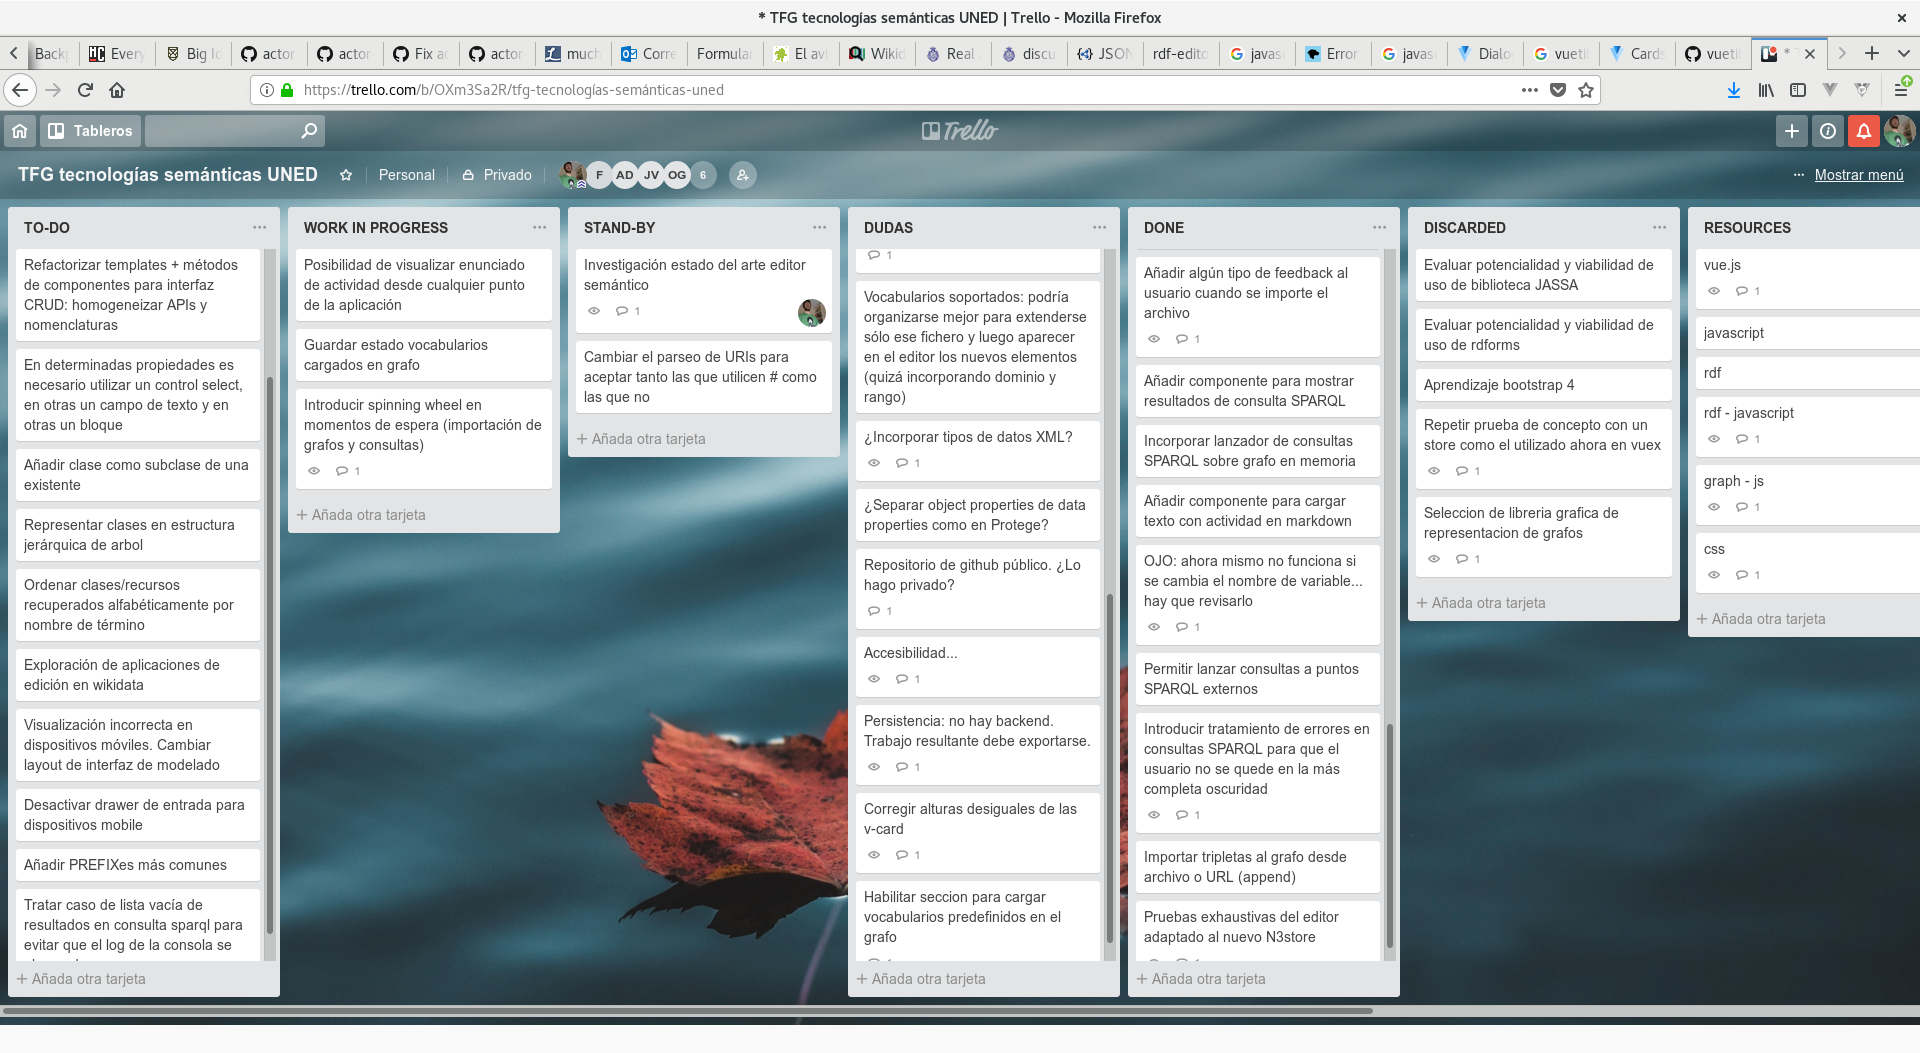
\includegraphics[scale=0.25]{trello}
	\caption{Ejemplo de tablero Trello}
\end{figure}

\cleardoublepage{}

\chapter{Recursos}

<....>\cleardoublepage{}

\chapter{An�lisis}

\section{Captura y documentaci�n de requisitos}

\subsection{Captura de requisitos}

La t�cnica de captura de requisitos utilizada para este proyecto ha sido, fundamentalmente, \textbf{la entrevista} con el tutor. Se eligi� esta t�cnica por los siguientes motivos:

\begin{itemize}  
	\item Las entrevistas, bien a distancia o presenciales (y especialmente estas �ltimas), permiten una mayor implicaci�n del usuario en la captura de requisitos.
	\item Combinada con una maqueta o prueba de concepto, una entrevista presencial puede dar lugar a la aparici�n de nuevos requisitos de producto, cambios en las especificaciones e incluso en el enfoque y objetivos del mismo.
	\item Permite la pr�ctica de la escucha activa y la sugerencia de ideas por parte del analista, aportando un valor a�adido que enriquece la simple captura de requisitos.
	\item Es claramente la t�cnica m�s obvia, directa y accesible en el contexto de la realizaci�n del proyecto.
\end{itemize}

Concretamente, se han llevado a cabo varias entrevistas utilizando la plataforma colaborativa Skype y una presencial, en la que el autor de este proyecto se ha desplazado a la sede del departamento en Madrid con objeto de conseguir una comunicaci�n m�s fluida y un mayor entendimiento a la hora de consensuar las necesidades y funcionalidades requeridas del producto.

La primera entrevista a distancia propici� un intercambio de documentos e ideas que desemboc� en la elaboraci�n del documento del anteproyecto. El resto de entrevistas a trav�s de Skype sirvieron para concretar en mayor medida las tareas a realizar y el enfoque del proyecto. Sin embargo, no fue hasta que no tuvo lugar la reuni�n presencial cuando realmente se le dio al proyecto su orientaci�n final, con unos objetivos claramente definidos y una posibilidad para cumplir los hitos propuestos.

A continuaci�n se resumen todas las sesiones de captura de requisitos:

\vspace*{\baselineskip}
\begin{center}
\begin{table}[htb]
\centering
\begin{tabular}{p{1cm}p{2cm}p{10cm}}
	\toprule
	id & Fecha & Resumen de la entrevista \\
	\toprule
	1 & 18/10/17 & Primer contacto y comunicaci�n de ideas iniciales para la confecci�n del anteproyecto  \\ \midrule
	2 & 21/02/17 & Consolidaci�n de ideas y aportaci�n de m�s documentaci�n (v�deos sobre prototipos de cuaderno, documentos de texto con descripciones, etc.)  \\
	3 & 28/03/18 & Primera demo a modo de POC con un entorno capaz de a�adir tripletas.  \\ \midrule
	4 & 10/07/18 & Reuni�n presencial con demostraci�n \textit{in-situ} de los m�dulos de modelado e importaci�n/exportaci�n. Tiene lugar una tormenta de ideas y se enfoca el proyecto de otro modo, modificando sus objetivos hacia una herramienta formativa..  \\ \midrule
	5 & 4/08/18 & Revisi�n de los �ltimos avances con la integraci�n de un endpoint SPARQL en el frontend y planificaci�n del resto de funcionalidade requeridas.  \\ 
	\bottomrule
\end{tabular}
\caption{Sesiones de entrevistas}
\label{tabmeetings}
\end{table}
\end{center}

\subsection{Documentaci�n}

Para documentar la captura de requisitos, se utilizar� la t�cnica de casos de uso. Se descarta la incorporaci�n de diagramas UML de casos de uso, dado que dichos diagramas carecen de informaci�n esencial sobre los mismos (como qu� actor lleva a cabo cada paso, o notas sobre el orden de ejecuci�n de los pasos). Si bien pueden ser �tiles como resumen o �ndice de contenidos, se decide prescindir de ellos dado que el n�mero de casos de uso contemplados en el proyecto es manejable.

Se utilizar� una plantilla propuesta por Cockburn{\cite{cockburn01}}: el estilo RUP (\textit{Rational Unified Process}){\cite{rational01}}, atractivo y f�cil de seguir pese al elevado n�mero de apartados, modificado para plasmar los aspectos m�s relevantes del proyecto (por ejemplo, no se incluir� un campo \textit{�mbito} porque siempre va a estar referido al mismo sistema o aplicaci�n). El motivo de no utilizar una tabla es meramente subjetivo, ya que el autor de esta memoria opina que puede oscurecer el contenido.

La plantilla sigue la siguiente estructura:

\begin{enumerate}  
	\item Nombre del caso de uso
	\begin{enumerate}
		\item Descripci�n breve
		\item Actores, entre los que estar� el actor principal. Presentan comportamiento.
		\item Disparadores: acciones sobre el sistema que inician los casos de uso.
	\end{enumerate}
	\item Flujo de eventos
		\begin{enumerate}
		\item Flujo b�sico: escenario principal de �xito.
		\item Flujos alternativos: qu� puede pasar que no sea el flujo principal.
			\begin{enumerate}
			\item Condicion 1
			\item Condici�n 2
			\item \ldots
		\end{enumerate}
	\end{enumerate}
	\item Requisitos especiales (si se dieran): plataforma, etc.
	\item Precondiciones: qu� debe ser cierto antes de ejecutar el caso de uso.
	\item Postcondiciones: qu� debe ser cierto despu�s de ejecutar el caso de uso.
\end{enumerate}

Los requisitos fueron capturados inicialmente como notas manuscritas y convertidos en necesidades de alto nivel en la plataforma Trello. A partir de ah�, dichas necesidades se refinaron para dar lugar a la bater�a de casos de uso incluida en \ref{sec:53}.

\section{Necesidades}

La reuni�n presencial marc� un punto de inflexi�n en cuanto a objetivos del proyecto, lo que se traduce en un cambio de necesidades. Para reflejar la evoluci�n completa, se dividir� su captura en dos fases detalladas a continuaci�n:

\subsection{Captura inicial}

A continuaci�n se resumen, en lenguaje natural, las necesidades identificadas durante la primera fase de desarrollo del proyecto:
\begin{enumerate}
\item Permitir a usuarios de la UNED  de distintos colectivos etiquetar y generar sus propios cuadernos con informaci�n y metainformaci�n sem�ntica.
\item Permitir a dichos usuarios realizar consultas sobre sus cuadernos.
\item Desarrollar una interfaz web que permita al usuario gestionar tripletas RDF.
\item Desarrollar un m�dulo de generaci�n de consultas SPARQL a partir de consultas de lectura y escritura en formato JSON.
\item Desarrollar los correspondientes productos de inter�s para el usuario: consultas exportadas en forma diversa (CSV, JSON) o embebidas en una plantilla HTML significativa para el usuario.
\item Ofrecer la posibilidad de variar interfaces de entrada y exportadores en funci�n de los distintos colectivos de usuario utilizando los metadatos sobre cuadernos RDF previamente almacenados en una base de datos relacional.
\item Permitir mostrar en pantalla una serie de t�rminos como punto de partida que el usuario pueda utilizar para construir ternas RDF y relaciones entre ellas.
\item Permitir mostrar en pantalla una serie de t�rminos como punto de partida que el usuario pueda utilizar para construir ternas RDF y relaciones entre ellas.
\item Ofrecer al usuario una visualizaci�n sencilla y correcta de su modelo que proporciona una perspectiva adecuada sobre la que trabajar.
\item Presentar una interfaz de mantenimiento del grafo: vocabulario e instancias (conceptualizaci�n y poblamiento de una ontolog�a).
\item Importar y exportar informaci�n estructurada en formatos sem�nticos est�ndar.
\item Extender con vocabularios tales como SKOS y OWL. 
\end{enumerate}

\subsection{Captura final}

Una vez celebrada la reuni�n presencial, se decidi� darle otro enfoque al proyecto. Si bien la idea inicial era desarrollar un sistema que permitiese generar cuadernos a trav�s de la manipulaci�n de grafos, una vez presentada una maqueta o prueba de concepto con funcionalidades b�sicas de modelado el tutor propuso convertir la herramienta en un \textit{playground} o sistema de realizaci�n de actividades acad�micas con un enfoque docente orientado a facilitar el aprendizaje de las tecnolog�as de la Web Sem�ntica (b�sicamente RDF y SPARQL) a personas con poco o ning�n contacto con estas materias (por ejemplo, alumnos de los Grados de Ingenier�a Inform�tica o en Tecnolog�as de la Informaci�n de la UNED).

Este nuevo enfoque se tradujo en la siguiente instant�nea de necesidades de alto nivel:

\begin{enumerate}
\item Permitir el modelado sem�ntico con edici�n CRUD de clases, subclases y propiedades de clases (anotaciones b�sicas).
\item Permitir la edici�n CRUD de relaciones o propiedades, subpropiedades, etc.
\item Ofrecer mecanismos de poblamiento del grafo.
\item Permitir el lanzamiento de consultas SPARQL sobre el grafo local y visualizaci�n de resultados.
\item Permitir el lanzamiento de consultas SPARQL sobre endpoints remotos y visualizaci�n de resultados.
\item Ofrecer funcionalidad de carga de consultas SPARQL predefinidas desde archivo de texto.
\item Incorporar m�dulo para a�adir un texto con la definici�n de la actividad a realizar en formato Markdown.
\item Permitir la importaci�n de tripletas desde archivos o URL.
\item Permitir la incorporaci�n (append) de tripletas al grafo local desde archivos o URL.
\item Ofrecer un panel para cargar en el grafo vocabularios comunes predefinidos.
\item Presentar una interfaz f�cil de usar y responsiva para el usuario, con una gesti�n de errores adecuada y suficiente.
\end{enumerate}

\section{Casos de uso} \label{sec:53}

\subsection{Dar de alta una nueva clase}

\subsubsection{Descripci�n breve}

Este caso de uso permite a un usuario a�adir una nueva clase a su grafo a trav�s de una tripleta que tendr� como sujeto el nombre de la clase, como objeto el recurso owl:Class y como predicado el recurso rdf:type. 

\subsubsection{Actores}

El actor principal es el usuario de la aplicaci�n (fundamentalmente dirigida a un alumno, pero podr�a ser un profesor o cualquier otro usuario).

\subsubsection{Disparadores}

El caso de usa comienza cuando el usuario pulsa en el bot�n flotante + asociado a la tarjeta del listado de clases.

\subsubsection{Flujo de eventos}
\begin{enumerate}
	\item Flujo b�sico
	\begin{enumerate}
		\item El usuario pulsa en el bot�n flotante + asociado a la tarjeta del listado de clases.
		\item Aparece un cuadro de di�logo donde el usuario debe introducir el nombre de la clase.
		\item El usuario introduce el URI del recurso que quiere dar de alta como clase y pulsa en guardar.
		\item El nuevo recurso de tipo clase se crea y aparece en el listado de clases.
	\end{enumerate}
	\item Flujo alternativo 1
\begin{enumerate}
	\item El usuario pulsa en el bot�n flotante + asociado a la tarjeta del listado de clases.
	\item Aparece un cuadro de di�logo donde el usuario debe introducir el nombre de la clase.
	\item El usuario introduce (o no) el URI del recurso que quiere dar de alta como clase y pulsa fuera del cuadro de di�logo.
	\item El cuadro de di�logo se cierra y no hay ning�n cambio en los recursos.
\end{enumerate}
	\item Flujo alternativo 2
	\begin{enumerate}
		\item El usuario pulsa en el bot�n flotante + asociado a la tarjeta del listado de clases.
		\item Aparece un cuadro de di�logo donde el usuario debe introducir el nombre de la clase.
		\item El usuario introduce el URI del recurso que quiere dar de alta como clase y pulsa en guardar.
		\item Ocurre un error en el guardado del recurso que le es comunicado al usuario a trav�s de una notificaci�n en pantalla.
	\end{enumerate}

\end{enumerate}

\subsubsection{Requisitos especiales}

Ninguno.

\subsubsection{Precondiciones}

El usuario debe haber navegado previamente hasta la secci�n de modelado, bien a trav�s de la pantalla de bienvenida, bien a trav�s de la barra de navegaci�n lateral.

\subsubsection{Postcondiciones}

Ninguna.

\subsubsection{Extensiones}

Ninguna.

\subsection{Editar una clase existente}

\subsubsection{Descripci�n breve}

Este caso de uso permite a un usuario editar el recurso asociado a una clase existente en su grafo y cambiar su URI.

\subsubsection{Actores}

El actor principal es el usuario de la aplicaci�n (fundamentalmente dirigida a un alumno, pero podr�a ser un profesor o cualquier otro usuario).

\subsubsection{Disparadores}

El caso de usa comienza cuando el usuario pulsa en el icono de men� asociado a la clase que quiere editar y selecciona la acci�n ``Editar''.

\subsubsection{Flujo de eventos}
\begin{enumerate}
	\item Flujo b�sico
	\begin{enumerate}
		\item El usuario pulsa en el icono de men� asociado a la clase que quiere editar y selecciona la acci�n ``Editar''.
		\item Aparece un cuadro de di�logo con el URI del recurso actual que el usuario puede modificar.
		\item El usuario modifica (o no) el URI del recurso  y pulsa en guardar.
		\item El recurso ha sido modificado y su cambio se ve reflejado en el listado.
	\end{enumerate}
\item Flujo alternativo 1
\begin{enumerate}
	\item El usuario pulsa en el icono de men� asociado a la clase que quiere editar y selecciona la acci�n ``Editar''.
	\item Aparece un cuadro de di�logo con el URI del recurso actual que el usuario puede modificar.
	\item El usuario modifica (o no) el URI del recurso  y pulsa fuera del cuadro de di�logo.
	\item El cuadro de di�logo se cierra y no hay ning�n cambio en los recursos.
\end{enumerate}
	\item Flujo alternativo 2
	\begin{enumerate}
		\item El usuario pulsa en el icono de men� asociado a la clase que quiere editar y selecciona la acci�n ``Editar''.
		\item Aparece un cuadro de di�logo con el URI del recurso actual que el usuario puede modificar.
		\item El usuario modifica (o no) el URI del recurso  y pulsa en guardar.
		\item Ocurre un error en el guardado del recurso que le es comunicado al usuario a trav�s de una notificaci�n en pantalla.
	\end{enumerate}
	
\end{enumerate}

\subsubsection{Requisitos especiales}

Ninguno.

\subsubsection{Precondiciones}

El usuario debe haber navegado previamente hasta la secci�n de modelado, bien a trav�s de la pantalla de bienvenida, bien a trav�s de la barra de navegaci�n lateral.

\subsubsection{Postcondiciones}

Ninguna.

\subsubsection{Extensiones}

Ninguna.

\subsection{Eliminar una clase existente}

\subsubsection{Descripci�n breve}

Este caso de uso permite a un usuario eliminar el recurso asociado a una clase existente en su grafo.

\subsubsection{Actores}

El actor principal es el usuario de la aplicaci�n (fundamentalmente dirigida a un alumno, pero podr�a ser un profesor o cualquier otro usuario).

\subsubsection{Disparadores}

El caso de usa comienza cuando el usuario pulsa en el icono de men� asociado a la clase que quiere editar y selecciona la acci�n ``Eliminar''.

\subsubsection{Flujo de eventos}
\begin{enumerate}
	\item Flujo b�sico
	\begin{enumerate}
		\item El usuario pulsa en el icono de men� asociado a la clase que quiere editar y selecciona la acci�n ``Eliminar''.
		\item Aparece un cuadro de di�logo advirtiendo al usuario de que si confirma el cambio, no podr� volver a recuperar el recurso del grafo.
		\item El usuario elige confirmar.
		\item El recurso y su detalle asociado desaparecen del listado.
	\end{enumerate}
\item Flujo alternativo 1
\begin{enumerate}
	\item El usuario pulsa en el icono de men� asociado a la clase que quiere editar y selecciona la acci�n ``Eliminar''.
	\item Aparece un cuadro de di�logo advirtiendo al usuario de que si confirma el cambio, no podr� volver a recuperar el recurso del grafo.
	\item El usuario pulsa fuera del cuadro de di�logo.
	\item El cuadro de di�logo se cierra y no hay ning�n cambio en los recursos.
\end{enumerate}
	\item Flujo alternativo 2
	\begin{enumerate}
		\item El usuario pulsa en el icono de men� asociado a la clase que quiere editar y selecciona la acci�n ``Eliminar''.
	\item Aparece un cuadro de di�logo advirtiendo al usuario de que si confirma el cambio, no podr� volver a recuperar el recurso del grafo.
	\item El usuario elige cancelar.
	\item El recurso y su detalle siguen apareciendo y no son eliminados.
	\end{enumerate}
	\item Flujo alternativo 3
\begin{enumerate}
	\item El usuario pulsa en el icono de men� asociado a la clase que quiere editar y selecciona la acci�n ``Eliminar''.
	\item Aparece un cuadro de di�logo advirtiendo al usuario de que si confirma el cambio, no podr� volver a recuperar el recurso del grafo.
	\item El usuario elige confirmar.
	\item  Ocurre un error en el borrado del recurso que le es comunicado al usuario a trav�s de una notificaci�n en pantalla.
\end{enumerate}
	
\end{enumerate}

\subsubsection{Requisitos especiales}

Ninguno.

\subsubsection{Precondiciones}

El usuario debe haber navegado previamente hasta la secci�n de modelado, bien a trav�s de la pantalla de bienvenida, bien a trav�s de la barra de navegaci�n lateral.

\subsubsection{Postcondiciones}

Una vez eliminada un recurso de tipo clase, se eliminan tambi�n todas las tripletas que lo tengan como objeto o como sujeto (es decir, cualquier relaci�n con dicha clase).

\subsubsection{Extensiones}

Ninguna.

\subsection{Dar de alta una nueva anotaci�n o propiedad est�ndar de una clase}

\subsubsection{Descripci�n breve}

Este caso de uso permite a un usuario a�adir una nueva propiedad de una clase a su grafo. Tan s�lo se podr�n a�adir propiedades entre las previamente configuradas en el c�digo fuente de la aplicaci�n (es decir, han de fijarse de manera previa, si bien su extensi�n es sencilla). La configuraci�n por defecto ofrece una lista de las propiedades m�s utilizadas.

\subsubsection{Actores}

El actor principal es el usuario de la aplicaci�n (fundamentalmente dirigida a un alumno, pero podr�a ser un profesor o cualquier otro usuario).

\subsubsection{Disparadores}

El caso de usa comienza cuando el usuario pulsa en el signo + asociado al nombre de la propiedad a la que quiere dar un valor.

\subsubsection{Flujo de eventos}
\begin{enumerate}
	\item Flujo b�sico
	\begin{enumerate}
		\item El usuario pulsa en el bot�n flotante + asociado a la tarjeta del listado de clases.
		\item Aparece un cuadro de di�logo donde el usuario debe introducir el nombre de la clase.
		\item El usuario introduce el URI del recurso que quiere dar de alta como clase y pulsa en guardar.
		\item El nuevo recurso de tipo clase se crea y aparece en el listado de clases.
	\end{enumerate}
	\item Flujo alternativo 1
	\begin{enumerate}
		\item El usuario pulsa en el bot�n flotante + asociado a la tarjeta del listado de clases.
		\item Aparece un cuadro de di�logo donde el usuario debe introducir el nombre de la clase.
		\item El usuario introduce (o no) el URI del recurso que quiere dar de alta como clase y pulsa fuera del cuadro de di�logo.
		\item El cuadro de di�logo se cierra y no hay ning�n cambio en los recursos.
	\end{enumerate}
	\item Flujo alternativo 2
	\begin{enumerate}
		\item El usuario pulsa en el bot�n flotante + asociado a la tarjeta del listado de clases.
		\item Aparece un cuadro de di�logo donde el usuario debe introducir el nombre de la clase.
		\item El usuario introduce el URI del recurso que quiere dar de alta como clase y pulsa en guardar.
		\item Ocurre un error en el guardado del recurso que le es comunicado al usuario a trav�s de una notificaci�n en pantalla.
	\end{enumerate}
	
\end{enumerate}

\subsubsection{Requisitos especiales}

Ninguno.

\subsubsection{Precondiciones}

El usuario debe haber navegado previamente hasta la secci�n de modelado, bien a trav�s de la pantalla de bienvenida, bien a trav�s de la barra de navegaci�n lateral, y haber seleccionado previamente una clase de entre el listado de clases (en la tarjeta de la izquierda) para poder a�adirle una propiedad.

\subsubsection{Postcondiciones}

Ninguna.

\subsubsection{Extensiones}

Ninguna.

\subsection{Editar una propiedad o anotaci�n de una clase}

\subsubsection{Descripci�n breve}

Este caso de uso permite a un usuario editar el recurso asociado a una propiedad o anotaci�n de una clase existente en su grafo y cambiar su URI. Tan s�lo se podr� editar una propiedad o anotaci�n de entre las previamente configuradas en el c�digo fuente de la aplicaci�n (es decir, han de fijarse de manera previa, si bien su extensi�n es sencilla).

\subsubsection{Actores}

El actor principal es el usuario de la aplicaci�n (fundamentalmente dirigida a un alumno, pero podr�a ser un profesor o cualquier otro usuario).

\subsubsection{Disparadores}

El caso de usa comienza cuando el usuario pulsa en el icono de men� asociado a la propiedad de clase que quiere editar y selecciona la acci�n ``Editar''.

\subsubsection{Flujo de eventos}
\begin{enumerate}
	\item Flujo b�sico
\begin{enumerate}
	\item El usuario pulsa en el icono de men� asociado a la propiedad de la clase que quiere editar y selecciona la acci�n ``Editar''.
	\item Aparece un cuadro de di�logo con el URI del recurso actual que el usuario puede modificar.
	\item El usuario modifica (o no) el URI del recurso  y pulsa en guardar.
	\item El recurso ha sido modificado y su cambio se ve reflejado en el listado de detalle de la propiedad.
\end{enumerate}
\item Flujo alternativo 1
\begin{enumerate}
	\item El usuario pulsa en el icono de men� asociado a la propiedad de la clase que quiere editar y selecciona la acci�n ``Editar''.
	\item Aparece un cuadro de di�logo con el URI del recurso actual que el usuario puede modificar.
	\item El usuario modifica (o no) el URI del recurso  y pulsa fuera del cuadro de di�logo.
	\item El cuadro de di�logo se cierra y no hay ning�n cambio en los recursos.
\end{enumerate}
\item Flujo alternativo 2
\begin{enumerate}
	\item El usuario pulsa en el icono de men� asociado a la propiedad de la clase que quiere editar y selecciona la acci�n ``Editar''.
	\item Aparece un cuadro de di�logo con el URI del recurso actual que el usuario puede modificar.
	\item El usuario modifica (o no) el URI del recurso  y pulsa en guardar.
	\item Ocurre un error en el guardado del recurso que le es comunicado al usuario a trav�s de una notificaci�n en pantalla.
	\end{enumerate}
	
\end{enumerate}

\subsubsection{Requisitos especiales}

Ninguno.

\subsubsection{Precondiciones}

El usuario debe haber navegado previamente hasta la secci�n de modelado, bien a trav�s de la pantalla de bienvenida, bien a trav�s de la barra de navegaci�n lateral, y haber seleccionado previamente una clase de entre el listado de clases (en la tarjeta de la izquierda) para poder editar una de sus propiedades a trav�s del men�.

\subsubsection{Postcondiciones}

Ninguna.

\subsubsection{Extensiones}

Ninguna.

\subsection{Eliminar una propiedad o anotaci�n de una clase}

\subsubsection{Descripci�n breve}

Este caso de uso permite a un usuario eliminar el recurso asociado a una propiedad o anotaci�n de una clase existente en su grafo. Tan s�lo se podr� eliminar una propiedad o anotaci�n de entre las previamente configuradas en el c�digo fuente de la aplicaci�n (es decir, han de fijarse de manera previa, si bien su extensi�n es sencilla).

\subsubsection{Actores}

El actor principal es el usuario de la aplicaci�n (fundamentalmente dirigida a un alumno, pero podr�a ser un profesor o cualquier otro usuario).

\subsubsection{Disparadores}

El caso de usa comienza cuando el usuario pulsa en el icono de men� asociado a la propiedad de clase que quiere editar y selecciona la acci�n ``Eliminar''.

\subsubsection{Flujo de eventos}
\begin{enumerate}
	\item Flujo b�sico
	\begin{enumerate}
		\item El usuario pulsa en el icono de men� asociado a la propiedad de la clase que quiere editar y selecciona la acci�n ``Eliminar''.
		\item Aparece un cuadro de di�logo advirtiendo al usuario de que si confirma el cambio, no podr� volver a recuperar el recurso del grafo.
	\item El usuario pulsa fuera del cuadro de di�logo.
	\item El cuadro de di�logo se cierra y no hay ning�n cambio en los recursos.
	\end{enumerate}
	\item Flujo alternativo 1
	\begin{enumerate}
		\item El usuario pulsa en el icono de men� asociado a la propiedad de la clase que quiere editar y selecciona la acci�n ``Eliminar''.
		\item Aparece un cuadro de di�logo advirtiendo al usuario de que si confirma el cambio, no podr� volver a recuperar el recurso del grafo.
	\item El usuario pulsa fuera del cuadro de di�logo.
	\item El cuadro de di�logo se cierra y no hay ning�n cambio en los recursos.
	\end{enumerate}
	\item Flujo alternativo 2
	\begin{enumerate}
		\item El usuario pulsa en el icono de men� asociado a la propiedad de la clase que quiere editar y selecciona la acci�n ``Editar''.
		\item Aparece un cuadro de di�logo advirtiendo al usuario de que si confirma el cambio, no podr� volver a recuperar el recurso del grafo.
	\item El usuario elige cancelar.
	\item El recurso y su detalle siguen apareciendo y no son eliminados.
	\end{enumerate}
	\item Flujo alternativo 3
\begin{enumerate}
	\item El usuario pulsa en el icono de men� asociado a la propiedad de la clase que quiere editar y selecciona la acci�n ``Eliminar''.
	\item Aparece un cuadro de di�logo advirtiendo al usuario de que si confirma el cambio, no podr� volver a recuperar el recurso del grafo.
	\item El usuario elige confirmar.
	\item  Ocurre un error en el borrado del recurso que le es comunicado al usuario a trav�s de una notificaci�n en pantalla.
\end{enumerate}
	
\end{enumerate}

\subsubsection{Requisitos especiales}

Ninguno.

\subsubsection{Precondiciones}

El usuario debe haber navegado previamente hasta la secci�n de modelado, bien a trav�s de la pantalla de bienvenida, bien a trav�s de la barra de navegaci�n lateral, y haber seleccionado previamente una clase de entre el listado de clases (en la tarjeta de la izquierda) para poder editar una de sus propiedades a trav�s del men�.

\subsubsection{Postcondiciones}

Ninguna.

\subsubsection{Extensiones}

Ninguna.

\subsection{Cargar una actividad}

\subsubsection{Descripci�n breve}

Este caso de uso permite a un usuario cargar en la aplicaci�n un fichero de texto en formato Markdown para su visualizaci�n. Su objetivo es presentar la actividad formativa a llevar a cabo en un formato legible y de forma persistente mientras se lleve a cabo la misma.

\subsubsection{Actores}

El actor principal es el usuario de la aplicaci�n (fundamentalmente dirigida a un alumno, pero podr�a ser un profesor o cualquier otro usuario).

\subsubsection{Disparadores}

El caso de usa comienza cuando el usuario pulsa en el bot�n de ``Importar archivo'' presente en la tarjeta de actividad.

\subsubsection{Flujo de eventos}
\begin{enumerate}
	\item Flujo b�sico
	\begin{enumerate}
		\item El usuario pulsa en el bot�n de ``Importar archivo'' presente en la tarjeta de actividad.
		\item Aparece un cuadro de di�logo para seleccionar un archivo en formato Markdown.
		\item El usuario selecciona un archivo en formato Markdown con extensi�n .md para cargar.
		\item El cuadro de di�logo se cierra y aparece un mensaje informando del �xito en la carga, dem�s de poderse visualizar el contenido de la actividad en la tarjeta de contenido de la misma.
	\end{enumerate}
	\item Flujo alternativo 1
	\begin{enumerate}
		\item El usuario pulsa en el bot�n de ``Importar archivo'' presente en la tarjeta de actividad.
		\item Aparece un cuadro de di�logo para seleccionar un archivo en formato Markdown.
		\item El usuario selecciona un archivo con una extensi�n distinta a .md para cargar.
		\item El cuadro de di�logo se cierra y aparece un mensaje de error informando de que solo es posible cargar archivos en formato Markdown (con extensi�n .md).
	\end{enumerate}
	\item Flujo alternativo 2
	\begin{enumerate}
		\item El usuario pulsa en el bot�n de ``Importar archivo'' presente en la tarjeta de actividad.
		\item El usuario selecciona un archivo en formato Markdown con extensi�n .md para cargar que ocupa m�s del m�ximo permitido (500K, siendo este m�ximo configurable)
		\item El cuadro de di�logo se cierra y aparece un mensaje de error informando de que solo es posible cargar archivos con tama�o inferior al m�ximo permitido, especificando cu�l es dicho m�ximo.
	\end{enumerate}
	
\end{enumerate}

\subsubsection{Requisitos especiales}

Ninguno.

\subsubsection{Precondiciones}

El usuario debe haber navegado previamente hasta la secci�n de Actividades a trav�s de la barra de navegaci�n lateral.

\subsubsection{Postcondiciones}

La actividad se visualizar� con el formato Markdown interpretado en HTML en la tarjeta asociada al contenido de la misma.

\subsubsection{Extensiones}

Ninguna.

\subsection{Cargar un vocabulario}

\subsubsection{Descripci�n breve}

Este caso de uso permite a un usuario cargar en la aplicaci�n los vocabularios m�s comunes de forma predefinida. Este conjunto de vocabularios es f�cilmente extensible a trav�s del c�digo fuente y se carga a trav�s de URLs externas.

\subsubsection{Actores}

El actor principal es el usuario de la aplicaci�n (fundamentalmente dirigida a un alumno, pero podr�a ser un profesor o cualquier otro usuario).

\subsubsection{Disparadores}

El caso de usa comienza cuando el usuario pulsa en uno de los interruptores asociado a cualquiera de los vocabularios m�s utilizados ofrecidos por la aplicaci�n, siempre y cuando dichos interruptores est�n en su posici�n ``desactivado''.

\subsubsection{Flujo de eventos}
\begin{enumerate}
	\item Flujo b�sico
	\begin{enumerate}
		\item El usuario pulsa en un interruptor inactivo de un vocabulario.
		\item El interruptor pasa a estar activo y el vocabulario cargado.
	\end{enumerate}
	\item Flujo alternativo 1
	\begin{enumerate}
		\item El usuario pulsa en un interruptor inactivo de un vocabulario.
		\item Ocurre un error al recuperar o cargar el vocabulario y el interruptor vuelve a su posici�n de desactivado. Simult�neamente, aparece un mensaje de error.
		
	\end{enumerate}
	
\end{enumerate}

\subsubsection{Requisitos especiales}

Es necesario que haya conexi�n a Internet para poder descargar los vocabularios de las URLs precargadas.

\subsubsection{Precondiciones}

El usuario debe haber navegado previamente hasta la secci�n de Vocabularios a trav�s de la barra de navegaci�n lateral.

\subsubsection{Postcondiciones}

Las tripletas de los vocabularios activados estar�n cargadas en el grafo junto con las del modelo.

\subsubsection{Extensiones}

Ninguna.

\subsection{Des-cargar un vocabulario}

\subsubsection{Descripci�n breve}

Este caso de uso permite a un usuario des-cargar en la aplicaci�n los vocabularios que haya podido cargar previamente. 

\subsubsection{Actores}

El actor principal es el usuario de la aplicaci�n (fundamentalmente dirigida a un alumno, pero podr�a ser un profesor o cualquier otro usuario).

\subsubsection{Disparadores}

El caso de usa comienza cuando el usuario pulsa en uno de los interruptores asociado a cualquiera de los vocabularios m�s utilizados ofrecidos por la aplicaci�n, siempre y cuando su posici�n est� en ``activado''.

\subsubsection{Flujo de eventos}
\begin{enumerate}
	\item Flujo b�sico
	\begin{enumerate}
		\item El usuario pulsa en un interruptor activo de un vocabulario.
		\item El interruptor pasa a estar inactivo y el vocabulario des-cargado.
	\end{enumerate}
	\item Flujo alternativo 1
	\begin{enumerate}
		\item El usuario pulsa en un interruptor activo de un vocabulario.
		\item Ocurre un error al recuperar o cargar el vocabulario para su borrado del grafo y el interruptor vuelve a su posici�n de ``activado'', puesto que el vocabulario no se ha podido des-cargar. Simult�neamente, aparece un mensaje de error.
		
	\end{enumerate}
	
\end{enumerate}

\subsubsection{Requisitos especiales}

Es necesario que haya conexi�n a Internet para poder descargar los vocabularios de las URLs precargadas y as� eliminarlos del grafo local.

\subsubsection{Precondiciones}

El usuario debe haber navegado previamente hasta la secci�n de Vocabularios a trav�s de la barra de navegaci�n lateral.

\subsubsection{Postcondiciones}

Las tripletas de los vocabularios desactivados ya no estar�n cargadas en el grafo junto con las del modelo.

\subsubsection{Extensiones}

Ninguna.

\subsection{Poblar el grafo con una tripleta}

\subsubsection{Descripci�n breve}

Este caso de uso permite a un usuario a�adir una tripleta arbitraria al grafo, seleccionando su sujeto (campo libre), predicado (campo de selecci�n que permite introducir nuevos t�rminos) y objeto  (campo de selecci�n que permite introducir nuevos t�rminos).

\subsubsection{Actores}

El actor principal es el usuario de la aplicaci�n (fundamentalmente dirigida a un alumno, pero podr�a ser un profesor o cualquier otro usuario).

\subsubsection{Disparadores}

El caso de usa comienza cuando el usuario comienza a rellenar los campos del formulario de poblamiento y pulsa en aceptar cuando ha terminado. 

\subsubsection{Flujo de eventos}
\begin{enumerate}
	\item Flujo b�sico
	\begin{enumerate}
		\item El usuario rellena los campos del formulario, bien con los selectores, bien con un texto libre.
		\item El usuario pulsa en a�adir instancia.
		\item Aparece un mensaje indicando el �xito de la operaci�n y la instancia se a�ade al grafo.
	\end{enumerate}
	\item Flujo alternativo 1
	\begin{enumerate}
		\item El usuario rellena los campos del formulario pero deja al menos un campo vac�o (sin rellenar).
		\item El usuario pulsa en a�adir instancia.
		\item Aparece un mensaje de error indicando que ning�n elemento de la terna puede ser nulo.
	\end{enumerate}
	
\end{enumerate}

\subsubsection{Requisitos especiales}

Para que las opciones del selector aparezcan precargadas es necesario que, adem�s de los recursos por defecto, se haya cargado alg�n tipo de modelo en el grafo.

\subsubsection{Precondiciones}

El usuario debe haber navegado previamente hasta la secci�n de Poblamiento a trav�s de la barra de navegaci�n lateral.

\subsubsection{Postcondiciones}

La terna a�adida en caso de �xito puede visualizarse utilizando el m�dulo de consultas o, en caso de ser una terna estructural de modelado, en el m�dulo correspondiente.

\subsubsection{Extensiones}

Ninguna.

\subsection{Importar grafo}

\subsubsection{Descripci�n breve}

Este caso de uso permite a un usuario importar un grafo completo en los formatos N3, Turtle, TriG o N-Triples. El grafo importado sustituir� al cargado por defecto en memoria por la aplicaci�n.

\subsubsection{Actores}

El actor principal es el usuario de la aplicaci�n (fundamentalmente dirigida a un alumno, pero podr�a ser un profesor o cualquier otro usuario).

\subsubsection{Disparadores}

El caso de usa comienza cuando el usuario importa un grafo desde archivo o desde URL.

\subsubsection{Flujo de eventos}
\begin{enumerate}
	\item Flujo b�sico
	\begin{enumerate}
		\item El usuario pulsa en importar desde archivo o rellena la URL del mismo y pulsa en el icono con forma de lupa.
		\item El usuario selecciona el archivo a importar en caso de ser importaci�n desde archivo.
		\item Aparece un mensaje indicando el �xito de la operaci�n y se carga el grafo en el almac�n.
	\end{enumerate}
	\item Flujo alternativo 1
	\begin{enumerate}
		\item  El usuario pulsa en importar desde archivo o rellena la URL del mismo y pulsa en el icono con forma de lupa.
		\item El usuario selecciona o apunta a un archivo que supera el l�mite de tama�o permitido (configurable en la aplicaci�n.)
		\item Aparece un mensaje de error indicando que no es posible cargar el grafo.
	\end{enumerate}
\item Flujo alternativo 2
\begin{enumerate}
	\item El usuario rellena la URL del mismo y pulsa en el icono con forma de lupa.
	\item La URL no est� disponible o devuelve un error de descarga (por ejemplo, CORS, si el servidor no est� preparado).
	\item Aparece un mensaje de error indicando que no es posible cargar el grafo.
\end{enumerate}
	
\end{enumerate}

\subsubsection{Requisitos especiales}

Para cargar archivos desde una URL externa, el servidor remoto tiene que tener correctamente configuradas las cabeceras CORS (\textit{Cross-Origin Resource Sharing})\footnote{\url{https://developer.mozilla.org/es/docs/Web/HTTP/Access_control_CORS}}

\subsubsection{Precondiciones}

El usuario debe haber navegado previamente hasta la secci�n de Importar/Exportar a trav�s de la barra de navegaci�n lateral.

\subsubsection{Postcondiciones}

Una vez cargado el grafo, este podr� visualizarse en el m�dulo de modelado (si tiene ternas estructurales) o en el de consulta en todo caso.

\subsubsection{Extensiones}

Ninguna.

\subsection{A�adir a grafo}

\subsubsection{Descripci�n breve}

Este caso de uso es una leve modificaci�n del anterior y permite a un usuario a�adir un grafo externo al ya existente en el almac�n en los formatos N3, Turtle, TriG o N-Triples. El grafo importado no sustituir� al cargado por defecto en memoria por la aplicaci�n, sino que pasar� a formar parte de �l.

\subsubsection{Actores}

El actor principal es el usuario de la aplicaci�n (fundamentalmente dirigida a un alumno, pero podr�a ser un profesor o cualquier otro usuario).

\subsubsection{Disparadores}

El caso de usa comienza cuando el usuario a�ade un grafo desde archivo o desde URL.

\subsubsection{Flujo de eventos}
\begin{enumerate}
	\item Flujo b�sico
	\begin{enumerate}
		\item El usuario pulsa en a�adir desde archivo o rellena la URL del mismo y pulsa en el icono con forma de lupa.
		\item El usuario selecciona el archivo a a�adir en caso de ser importaci�n desde archivo.
		\item Aparece un mensaje indicando el �xito de la operaci�n y se a�ade el grafo en el almac�n.
	\end{enumerate}
	\item Flujo alternativo 1
	\begin{enumerate}
		\item  El usuario pulsa en a�adir a archivo o rellena la URL del mismo y pulsa en el icono con forma de lupa.
		\item El usuario selecciona o apunta a un archivo que supera el l�mite de tama�o permitido (configurable en la aplicaci�n.)
		\item Aparece un mensaje de error indicando que no es posible cargar el grafo.
	\end{enumerate}
	\item Flujo alternativo 2
	\begin{enumerate}
		\item El usuario rellena la URL del mismo y pulsa en el icono con forma de lupa.
		\item La URL no est� disponible o devuelve un error de descarga (por ejemplo, CORS, si el servidor no est� preparado).
		\item Aparece un mensaje de error indicando que no es posible a�adir el grafo.
	\end{enumerate}
	
\end{enumerate}

\subsubsection{Requisitos especiales}

Para cargar archivos desde una URL externa, el servidor remoto tiene que tener correctamente configuradas las cabeceras CORS (\textit{Cross-Origin Resource Sharing})\footnote{\url{https://developer.mozilla.org/es/docs/Web/HTTP/Access_control_CORS}}

\subsubsection{Precondiciones}

El usuario debe haber navegado previamente hasta la secci�n de Importar/Exportar a trav�s de la barra de navegaci�n lateral.

\subsubsection{Postcondiciones}

Una vez a�adido el grafo, este podr� visualizarse junto con el existente previamente en el m�dulo de modelado (si tiene ternas estructurales) o en el de consulta en todo caso.

\subsubsection{Extensiones}

Ninguna.

\subsection{Exportar grafo}

\subsubsection{Descripci�n breve}

Este caso de uso  permite a un usuario exportar a un archivo de texto en formato Turtle o JSON-LD el grafo de trabajo.

\subsubsection{Actores}

El actor principal es el usuario de la aplicaci�n (fundamentalmente dirigida a un alumno, pero podr�a ser un profesor o cualquier otro usuario).

\subsubsection{Disparadores}

El caso de usa comienza cuando el usuario pulsa en el bot�n de ``Exportar JSON-LD'' o ``Exportar Turtle''.

\subsubsection{Flujo de eventos}
\begin{enumerate}
	\item Flujo b�sico
	\begin{enumerate}
		\item El usuario pulsa en el bot�n de ``Exportar JSON-LD'' o ``Exportar Turtle''.
		\item El grafo se exporta y aparece un cuadro de di�logo para guardar el archivo.
	\end{enumerate}
	\item Flujo alternativo 1
	\begin{enumerate}
		\item El usuario pulsa en el bot�n de ``Exportar JSON-LD'' o ``Exportar Turtle''.
		\item Ocurre un error inesperado que se muestra al usuario.
	\end{enumerate}
	
\end{enumerate}

\subsubsection{Requisitos especiales}

Ninguno.

\subsubsection{Precondiciones}

Debe existir un grafo cargado en memoria.

\subsubsection{Postcondiciones}

Ninguna.

\subsubsection{Extensiones}

Ninguna.

\subsection{Lanzar consulta a grafo local}

\subsubsection{Descripci�n breve}

Este caso de uso  permite a un usuario lanzar una consulta SPARQL al grafo local cargado en memoria, bien desde un archivo con extensi�n ``rq'' o URL, bien desde un cuadro de texto.

\subsubsection{Actores}

El actor principal es el usuario de la aplicaci�n (fundamentalmente dirigida a un alumno, pero podr�a ser un profesor o cualquier otro usuario).

\subsubsection{Disparadores}

El caso de usa comienza cuando el usuario carga la consulta pulsa en el bot�n de ``Lanzar Consulta''.

\subsubsection{Flujo de eventos}
\begin{enumerate}
	\item Flujo b�sico
	\begin{enumerate}
		\item El usuario carga la consulta a lanzar, bien escribi�ndola en el cuadro de texto, bien carg�ndola desde un archivo ``rq'' o URL donde se encuentre.
		\item El usuario pulsa en el bot�n de ``Lanzar Consulta''.
		\item Los resultados de la consulta aparecen en la tabla de ``Resultados''.
		
	\end{enumerate}
	\item Flujo alternativo 1
	\begin{enumerate}
			\item El usuario carga la consulta a lanzar, bien escribi�ndola en el cuadro de texto, bien carg�ndola desde un archivo ``rq'' o URL donde se encuentre.
		\item El usuario pulsa en el bot�n de ``Lanzar Consulta''.
		\item Ocurre un error inesperado o de sintaxis al lanzar la consulta y aparece un mensaje de error para el usuario.
	\end{enumerate}
	
\end{enumerate}

\subsubsection{Requisitos especiales}

Ninguno.

\subsubsection{Precondiciones}

Debe existir un grafo cargado en memoria.

\subsubsection{Postcondiciones}

Ninguna.

\subsubsection{Extensiones}

Ninguna.

\subsection{Lanzar consulta a grafo remoto}

\subsubsection{Descripci�n breve}

Este caso de uso  permite a un usuario lanzar una consulta SPARQL a un grafo ubicado en un endpoint remoto, bien desde un archivo con extensi�n ``rq'' o URL, bien desde un cuadro de texto.

\subsubsection{Actores}

El actor principal es el usuario de la aplicaci�n (fundamentalmente dirigida a un alumno, pero podr�a ser un profesor o cualquier otro usuario).

\subsubsection{Disparadores}

El caso de usa comienza cuando el usuario activa la opci�n ``Usar endpoint SPARQL remoto''.

\subsubsection{Flujo de eventos}
\begin{enumerate}
	\item Flujo b�sico
	\begin{enumerate}
		\item El usuario activa la opci�n ``Usar endpoint SPARQL remoto''.
		\item El usuario introduce la URL del endpoint remoto.
		\item El usuario carga la consulta a lanzar, bien escribi�ndola en el cuadro de texto, bien carg�ndola desde un archivo ``rq'' o URL donde se encuentre.
		\item El usuario pulsa en el bot�n de ``Lanzar Consulta''.
		\item Los resultados de la consulta al grafo remoto aparecen en la tabla de ``Resultados''.
		
	\end{enumerate}
	\item Flujo alternativo 1
	\begin{enumerate}
		\item El usuario activa la opci�n ``Usar endpoint SPARQL remoto''.
		\item El usuario introduce la URL del endpoint remoto.
		\item El usuario carga la consulta a lanzar, bien escribi�ndola en el cuadro de texto, bien carg�ndola desde un archivo ``rq'' o URL donde se encuentre.
		\item El usuario pulsa en el bot�n de ``Lanzar Consulta''.
		\item Ocurre un error inesperado, de URL o de sintaxis al lanzar la consulta y aparece un mensaje de error para el usuario.
	\end{enumerate}
	
\end{enumerate}

\subsubsection{Requisitos especiales}

Ninguno.

\subsubsection{Precondiciones}

Los endpoints remotos deben soportar el protocolo SPARQL y tener correctamente configuradas las cabeceras CORS.

\subsubsection{Postcondiciones}

Ninguna.

\subsubsection{Extensiones}

Ninguna.\cleardoublepage{}

\include{dise�o}\cleardoublepage{}

\chapter{Implementaci�n}

<....>\cleardoublepage{}

\chapter{Pruebas}

<....>\cleardoublepage{}

\chapter{Resultados}

<....>\cleardoublepage{}

\chapter{Conclusiones y l�neas de trabajo futuras}


\section{Conclusiones}

Alimentar la Web con datos estructurados y contextualizados con metadatos no ha de ser una labor exclusiva de entornos acad�micos y universitarios. Si bien son estas organizaciones las que han modelado dominios de informaci�n y liberado conjuntos de datos de forma masiva a lo largo de los �ltimos a�os, es necesario extender esta responsabilidad a otros organismos p�blicos y privados y, por qu� no, a potenciales usuarios o clientes particulares. Solo a partir de ese momento, el relato inicial de Berners-Lee\cite{bernerslee01} en su primera definici�n de la Web Sem�ntica ser� una realidad en nuestra Sociedad.

No obstante, a�n queda mucho trabajo por hacer. Organizaciones p�blicas y privadas han de concienciarse de la enorme importancia de poner a disposici�n de la Sociedad en general datos estructurados en formatos reutilizables. S�lo de esta forma crecer� el inter�s en su tratamiento y explotaci�n, as� como en el desarrollo de agentes inteligentes que sean capaz de procesarlos para generar nuevos resultados de an�lisis. No hay m�s que recurrir a los datos del Estudio de Caracterizaci�n del Sector Infomediario en Espa�a\cite{ontsi01} proporcionados por el Observatorio Nacional de las Telecomunicaciones y de la Sociedad de la Informaci�n, que recogen que el 70\% de las empresas encuestadas accede a datos no estructurados, frente al 69\% que lo hace a datos en formatos abiertos (si bien no se especifica si se trata de datos a nivel de datos abiertos enlazados o \textit{linked open data}).

La comunidad de tecnol�gos y desarrolladores de aplicaciones para la Web Sem�ntica debe trabajar por la democratizaci�n de esta tecnolog�a. Con los niveles de complejidad conceptual y de uso actuales, su difusi�n entre el p�blico general se hace complicada. En este sentido, las grandes revoluciones surgidas en torno al mundo del desarrollo de \textit{frontend} web en general (y \textit{Javascript} en particular) y el nivel de madurez alcanzado en estos momentos por las tecnolog�as de la Web Sem�ntica, favorecen la llegada del momento m�s propicio en los �ltimos veinte a�os para lograr un impulso real. A�n son pocas las comunidades de desarrolladores trabajando en ofrecer servicios sem�nticos a trav�s de \textit{Javascript}, pero la existencia de un \textit{``community group''}\cite{rdfw3ccg} que aglutina esfuerzos para aunar a dichas comunidades en un s�lo proyecto es una noticia prometedora de cara al futuro de esta tecnolog�a.

Como peque�a contribuci�n a estos esfuerzos de difusi�n y democratizaci�n, se ha desarrollado el presente proyecto, que representa la culminaci�n de meses de trabajo pero tambi�n el inicio de la vida de un producto. Se sientan las bases para obtener una herramienta acad�mica que permita acercar las tecnolog�as de la Web Sem�ntica a cualquier no iniciado. Si bien en esta primera versi�n ya se cuenta con una aplicaci�n funcional, el estado de las bibliotecas que integra y las posibilidades de RDF y SPARQL sugieren unas expectativas de evoluci�n lo suficientemente optimistas como para continuar su desarrollo y no abandonar su mantenimiento.

A partir de este punto, la hoja de ruta que se propone para el producto desarrollado en el presente proyecto es clara: en un primer curso acad�mico, comenzar a utilizarlo a modo de prueba piloto en asignaturas t�cnicas relacionadas con la Web Sem�ntica a trav�s de actividades opcionales (para mejorar la nota total del alumno, por ejemplo) e ir evaluando su idoneidad de cara a su manejo en el entorno para el que fue pensado. Paralelamente, la aplicaci�n puede seguir siendo mejorada y perfeccionada, en caso de aparici�n de defectos inesperados (algo, por otra parte, perfectamente asumible hoy en d�a).

Un claro compromiso por parte del autor del proyecto debe ser para con la Comunidad Educativa, y especialmente para los grupos de trabajo como el \textit{RDF Javascript Libraries Community Group} por su inestimable ayuda prestada. Por tanto, parece razonable trabajar en una futura traducci�n al idioma ingl�s para permitir su publicaci�n como repositorio de c�digo abierto y revertir el desarrollo a la Comunidad.

No se podr�a concluir este cap�tulo de conclusiones sin valorar las competencias tecnol�gicas y organizativas que el desarrollo del proyecto ha permitido adquirir a su autor: profundizaci�n en el modelado RDF, las arquitecturas de aplicaciones de la Web Sem�ntica, los motores de consultas SPARQL y el desarrollo en marcos de trabajo \textit{Javascript} completos y bien estructurados como Vue.js (una inversi�n, esta �ltima, m�s que rentable en t�rminos de utilizaci�n de la tecnolog�a).

Tomar decisiones entre altas dosis de incertidumbre no es sencillo, y menos a�n cuando la oferta tecnol�gica es numerosa y variada (como es el caso, por ejemplo, de las bibliotecas de componentes gr�ficos para Vue). Adem�s, la complejidad inicial del desarrollo en \textit{Javascript} no presenta una curva de aprendizaje suave, especialmente en la configuraci�n del entorno necesario: empaquetadores, \textit{``transpilers''} con sus m�dulos asociados, existencia de diversos est�ndares conviviendo entre distintos m�dulos que complican su integraci�n, etc.

Por otra parte, los trabajos previos de implementaci�n de RDF en \textit{Javascript} tambi�n son numerosos y confusos (prueba de ello es la reciente noticia de Junio de este mismo a�o, 2018, indicando la unificaci�n de las diferentes implementaciones existentes en una �nica implementaci�n). Afortunadamente, la ayuda y los consejos de los propios desarrolladores, ya con experiencia, ha permitido enfocar el proyecto con las estrategias adecuadas.

En resumidas cuentas, se ha tratado de obtener un producto apto para la formaci�n acad�mica en tecnolog�as de la Web Sem�ntica, cumpliendo razonablemente con los objetivos iniciales y abriendo un camino al desarrollo de una herramienta mucho m�s completa que pueda aprovecharse de las tecnolog�as emergentes en el �rea del \textit{frontend} web. Se han utilizado bibliotecas y m�dulos est�ndares dentro de la situaci�n actual, lo que permitir� una mayor facilidad de mantenimiento en el futuro y pretende abrir el camino a evoluciones m�s ambiciosas. A fecha de finalizaci�n de la presente memoria, ya se est�n manteniendo conversaciones con el Director del Proyecto para el futuro uso de la aplicaci�n en la actividad docente, lo que permitir�, sin duda, obtener \textit{feedback} de cara a su futura mejora. El tablero Kanban del proyecto y el propio repositorio en Github est�n disponibles desde este momento para incorporar nuevas tarjetas y peticiones de evoluci�n o mejora.

\section{L�neas de trabajo futuras}

Como punto de partida para futuras mejoras y nuevas funcionalidades, se proponen las siguientes l�neas de trabajo:

\begin{itemize}
\item Integrar la primera versi�n estable (una vez publicada) de los distintos m�dulos de la plataforma Comunica y optimizar el uso de dependencias.
\item Integrar las futuras versiones del marco de trabajo de componentes Vuetify y utilizar nuevos componentes como la estructura jer�rquica (en �rbol) para representar clases y propiedades.
\item Integrar o desarrollar consultas SPARQL con Comunica a grafos en RDFXML\footnote{\url{https://github.com/comunica/comunica/issues/140}}
\item Incrementar la cobertura de pruebas unitarias y extremo a extremo
\item Re-orientar las operaciones de consulta a trav�s del m�dulo \textit{actor-init-sparql-rdfjs} (ver secci�n \ref{sec:motor-de-consultas-en-el-proyecto})
\item Funcionalidad de exportar a un formato JSON-raw (una lista de objetos con ternas).
\item Posibilidad de modificar los prefijos a incluir en las consultas. En general, facilitar el uso de prefijos.
\item Enriquecer y refactorizar la funcionalidad de modelado.
\item Soportar m�ltiples grafos.
\item Revisar la carga de t�rminos b�sicos y estudiar la viabilidad de carga en l�nea desde una ontolog�a est�ndar.
\item Traducci�n de la aplicaci�n al idioma ingl�s y puesta a disposici�n de las distintas comunidades de desarrolladores y usuarios.
\end{itemize} 


\cleardoublepage{}\fancyhead[LO]{\nouppercase{\leftmark}}\fancyhead[RE]{\nouppercase{\rightmark}}

\cleardoublepage{}

\bibliographystyle{unsrt}
\bibliography{biblio/biblio-pfg}


\appendix
\cleardoublepage{}\renewcommand{\appendixname}{Anexo}

\chapter{Manual de usuario}

El manual de usuario forma parte de la propia aplicaci�n web, pudiendo ser accedido a trav�s del enlace ``Ayuda'' ubicado en el pie de p�gina de la misma.



\end{document}
